%
% teil2.tex -- Beispiel-File für teil2 
%
% (c) 2020 Prof Dr Andreas Müller, Hochschule Rapperswil
%
% !TEX root = ../../buch.tex
% !TEX encoding = UTF-8
%
\section{Oszilierende Muster
\label{reaktdiff:section:teil2}}
\kopfrechts{Teil 2}
Zum Schluss dieses Papers werden Systeme beleuchtet, welche oszillieren.
Hierfür wird die Lotka-Volterra-Reaktion als Beispiel genommen.


\subsection{Lotka-Volterra Reaktion 
\label{reaktdiff:subsection:bonorum}}

Die Lotka-Volterra Reaktion \cite{Wikipedia_LotkaVolterra_2025}  besteht ebenfalls wie die Turing-Muster aus einem Reaktionsdiffusionsmodell mit zwei Gleichungen.
Der grosse Unterschied zu den Turing-Mustern ist, dass die Lotka-Volterra-Reaktion bereits ohne Diffusion instabil ist.
Die Lotka-Volterra-Reaktion (oder Gleichung) wird ebenfalls benutzt, um das klassische Räuber-Beute-Modell zu beschreiben.

\subsubsection{Mathematik hinter der Lotka-Volterra Reaktion}

Wieder werden \(u(x,t)\) und \(v(x,t)\) verwendet um die Konzentration an einem bestimmten Ort zu einem bestimmten Zeitpunkt zu beschreiben.
Die Reaktionsterme
\begin{equation}
     f(u,v) = \alpha u -  \beta v, \quad g(u,v)= \delta uv - \gamma
      \label{reaktdiff:equation:lvsys}
\end{equation}
bestehen neben den Konzentration \(u,v\) aus den Konstanten \(\alpha\),\(\beta\), \(\delta\) und \(\gamma\).

Das dazugehörige Reaktionsdiffusionssystem
\begin{align*}
    \frac{\partial u}{\partial t} &= D_u \Delta u + \alpha u - \beta u v,
    %\label{reaktdiff:equation:lv1}
    \\
    \frac{\partial v}{\partial t} &= D_v \Delta v + \delta u v - \gamma v
    %\label{reaktdiff:equation:lv2}
\end{align*}
besteht wieder aus \(D_u,D_v > 0\).
Das System hat Nullstellen bei  \(u = 0,v = 0\) (trivial) und bei \(u = \frac{\gamma}{\delta}, v = \frac{\alpha}{\beta}\).
Um die Stabilität an diesen Punkten zu untersuchen, wird wie auch zuvor im Kapitel das System linearisiert und an der interessanten Nullstelle untersucht.
Die Jacobi-Matrix des Systems lautet
\begin{equation*}
        J(u,v) =
        \begin{pmatrix}
        \frac{\partial f}{\partial u} & \frac{\partial f}{\partial v} \\
        \frac{\partial g}{\partial u} & \frac{\partial g}{\partial v}
        \end{pmatrix}
        =
        \begin{pmatrix}
        \alpha - \beta v & -\beta u \\
        \delta v & \delta u - \gamma
        \end{pmatrix}.
\end{equation*}
An der Stelle \(u = \frac{\gamma}{\delta}, v = \frac{\alpha}{\beta}\) ergibt das
\begin{equation*}
         J\left(\frac{\gamma}{\delta},\frac{\alpha}{\beta}\right) =
        \begin{pmatrix}
        0 & -\beta \cdot\frac{\gamma}{\delta} \\
        \delta \cdot \frac{\alpha}{\beta} & 0
        \end{pmatrix}. 
\end{equation*}
Somit erhält man
\begin{equation*}
    \lambda^2 + \sqrt{\frac{\delta \alpha \cdot \beta \gamma}{\delta \beta}}
     = 
     \lambda^2 + \alpha \gamma = 0 
     \Rightarrow
     \lambda = \pm j \sqrt{a\gamma}
\end{equation*}
als Eigenwerte.
Die Eigenwerte sind rein imaginär.
Das bedeutet, dass eine kleine Störung im System keine Dämpfung erfährt.
Es entsteht ein oszillierendes Muster (siehe Abbildung \ref{reaktdiff:fig:lv}).

\subsubsection{Simulation der LV-Reaktion}

Für die Simulation werden die Werte \(\alpha = 1, \beta = 0.1, \gamma = 1.5, \delta = 0.75\) verwendet.
Somit befindet sich das Gleichgewicht bei
\begin{equation*}
    u = \frac{\gamma}{\delta} = \frac{1.5}{0.75} = 2, 
    v = \frac{\alpha}{\beta} = \frac{1}{0.1} = 10.
\end{equation*}
Die Eigenwerte haben den Betrag \(\omega = \sqrt{\alpha\gamma} = \sqrt{1 \cdot 1.5} \approx 1.225\).
Die FFT der Simulation ist in Abbildung \ref{reaktdiff:fig:lvfft} zu sehen.
Die rote Linie zeigt die berechnete Frequenz \(f = \omega / 2 \pi \approx 0.195\,\text{Hz}\).
In der Grafik sieht man, dass die berechnete Frequenz nicht ganz mit der dominanten Frequenz der Simulation übereinstimmt.
Diese Abweichung kann durch numerische Effekte erklärt werden.

\begin{figure}
    \centering
    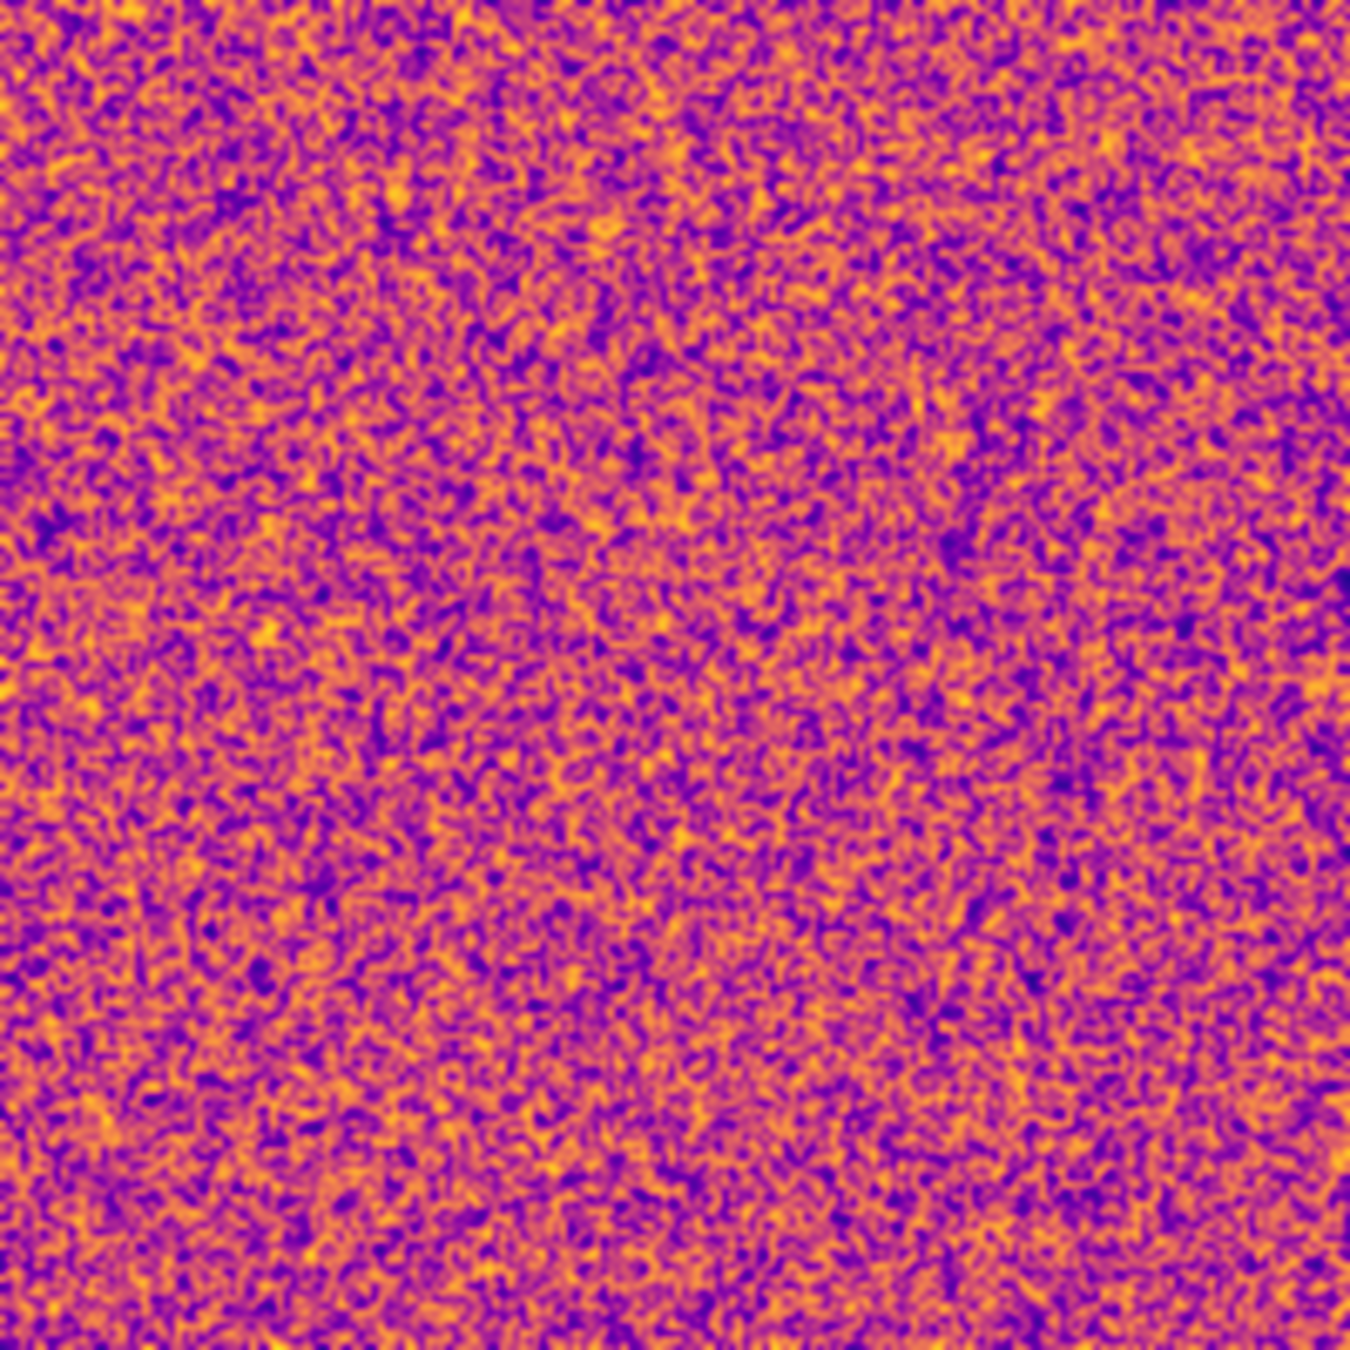
\includegraphics[width=0.32\linewidth]{papers/reaktdiff/images/LotkaVolterra/lv_n1.png}
    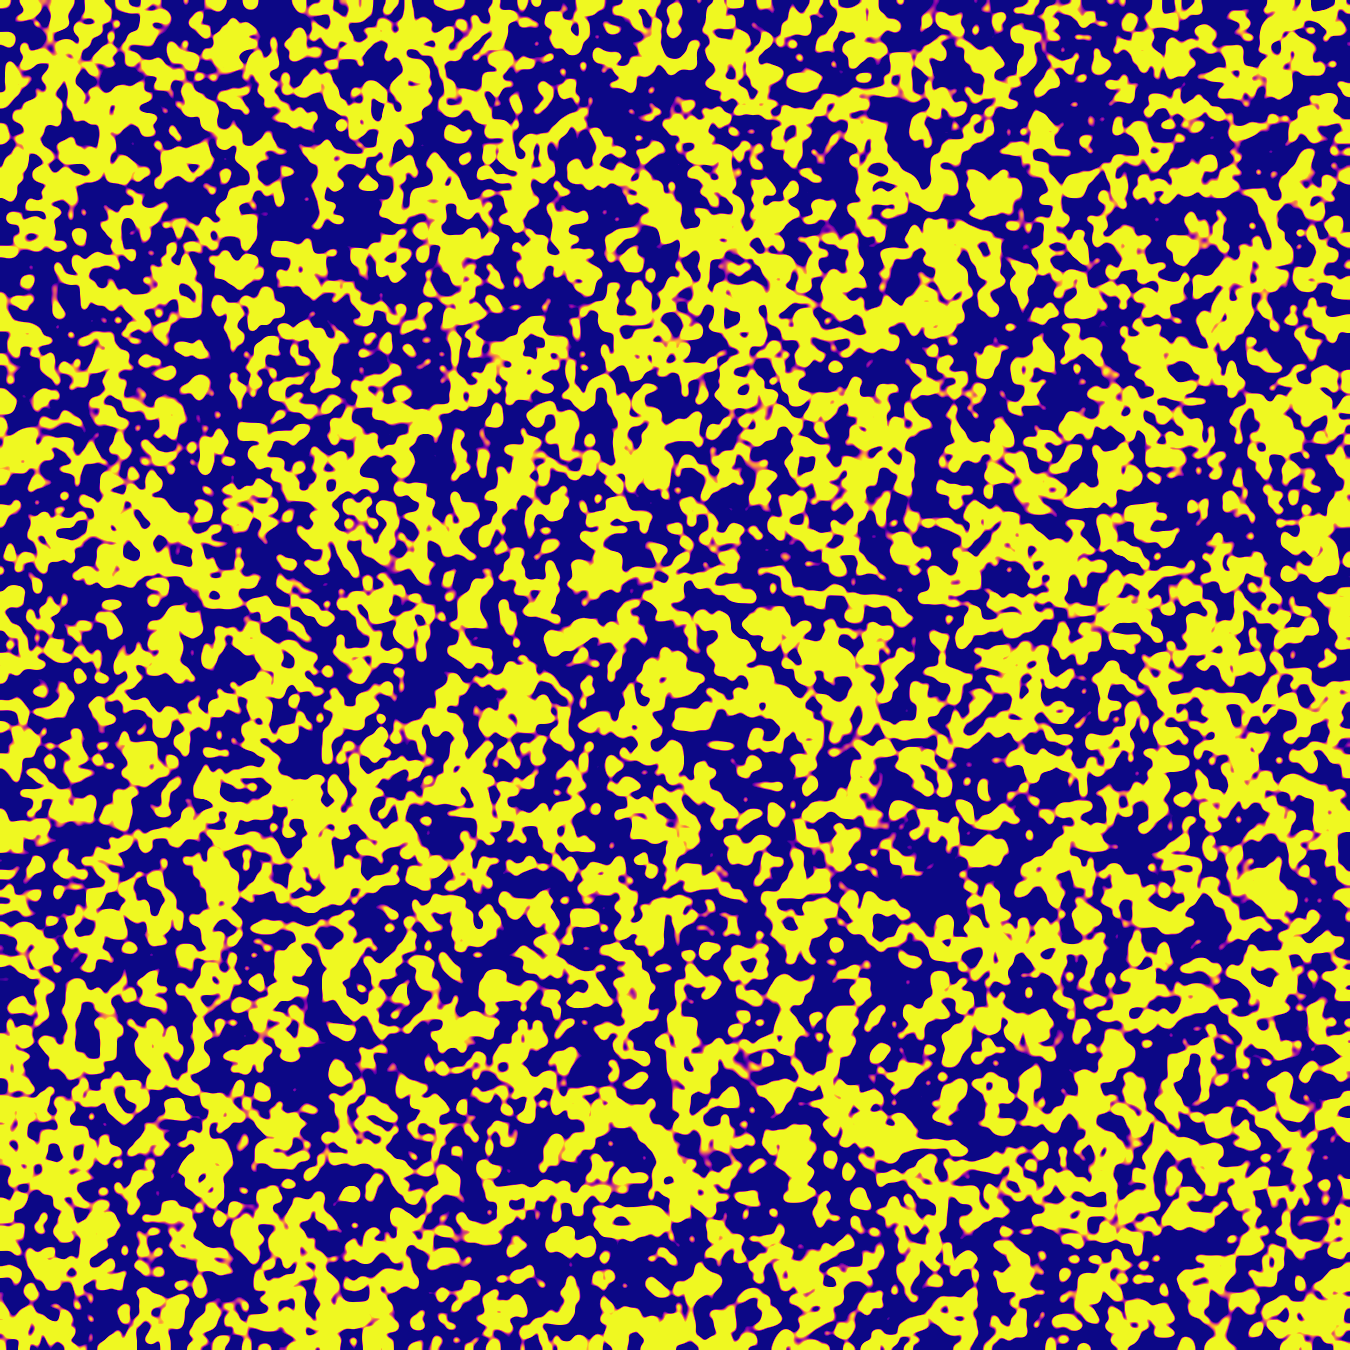
\includegraphics[width=0.32\linewidth]{papers/reaktdiff/images/LotkaVolterra/lv_n300.png}
    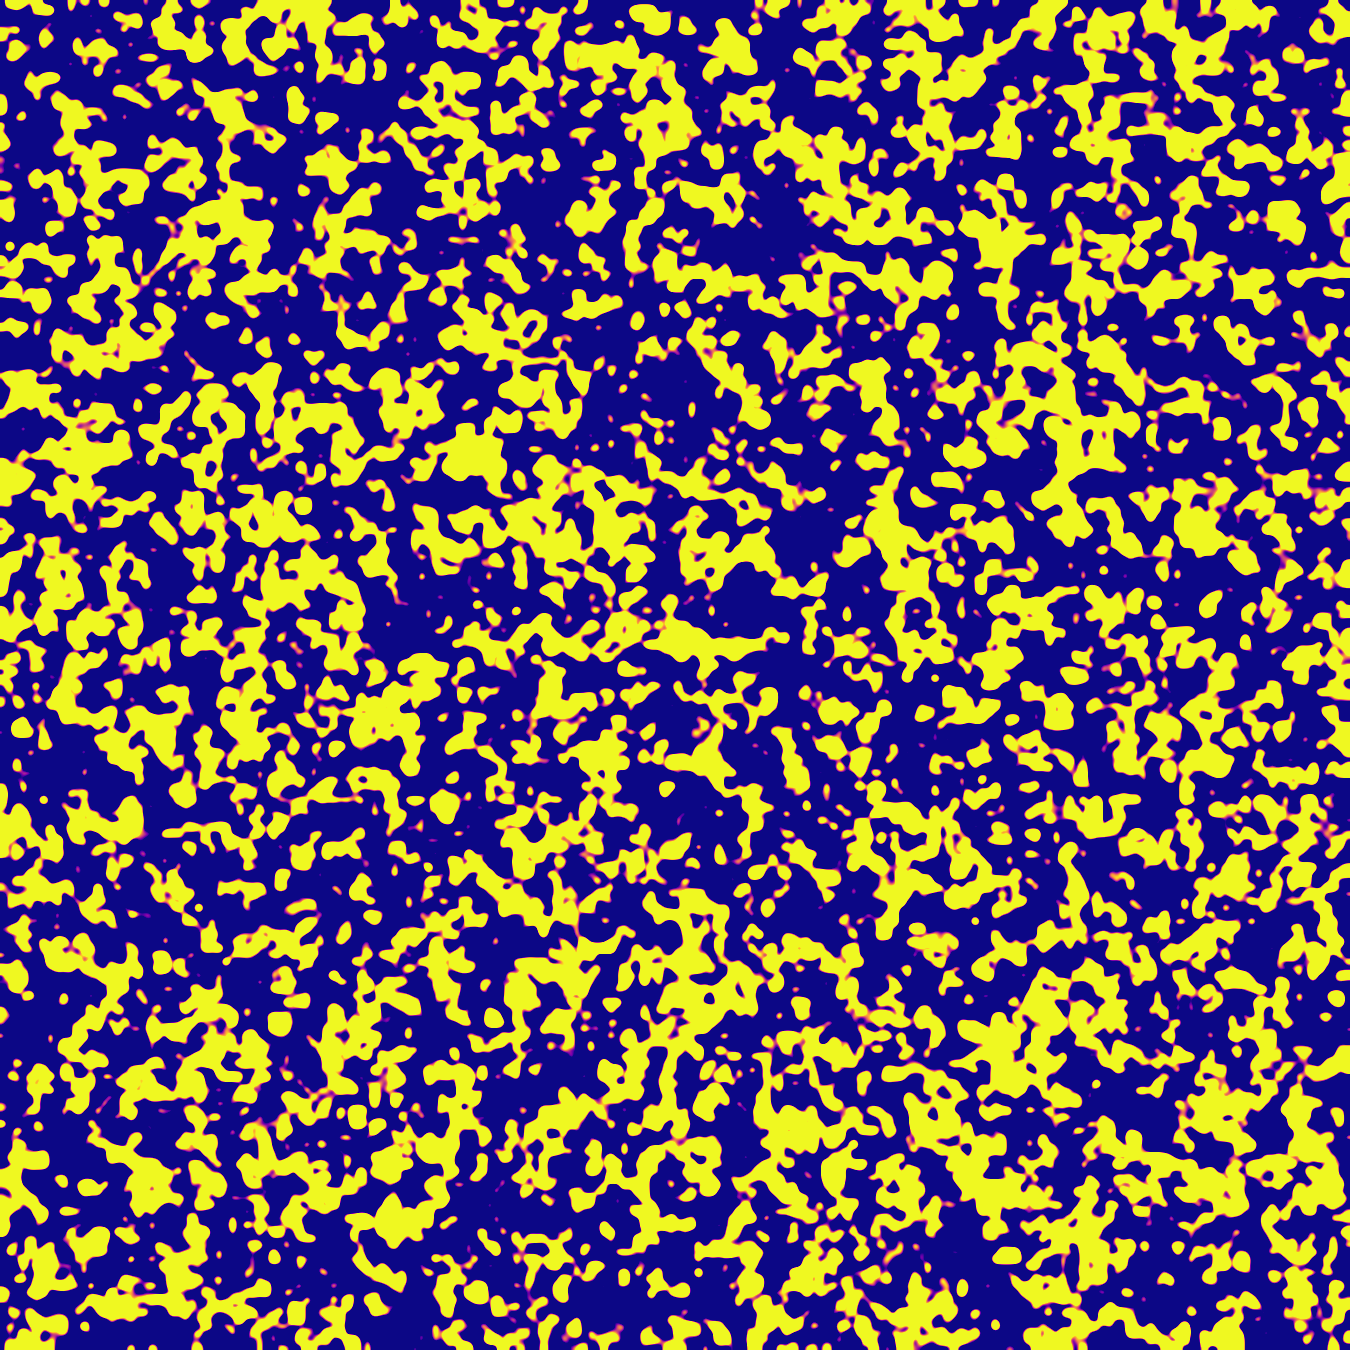
\includegraphics[width=0.32\linewidth]{papers/reaktdiff/images/LotkaVolterra/lv_n999.png}
    \caption{Verlauf der Simulation (links nach rechts) der Reaktions-Diffusiongleichung mit Lotka-Volterra Modell \eqref{reaktdiff:equation:lvsys}
     als Reaktionsterm. Die erste Grafik zeigt den Anfangszustand. Die Oszillation ist in den Grafiken 2 und 3 angedeutet, jedoch schwer mit statischen Bilder darzustellen.}
    \label{reaktdiff:fig:lv}
\end{figure}

\begin{figure}
    \centering
    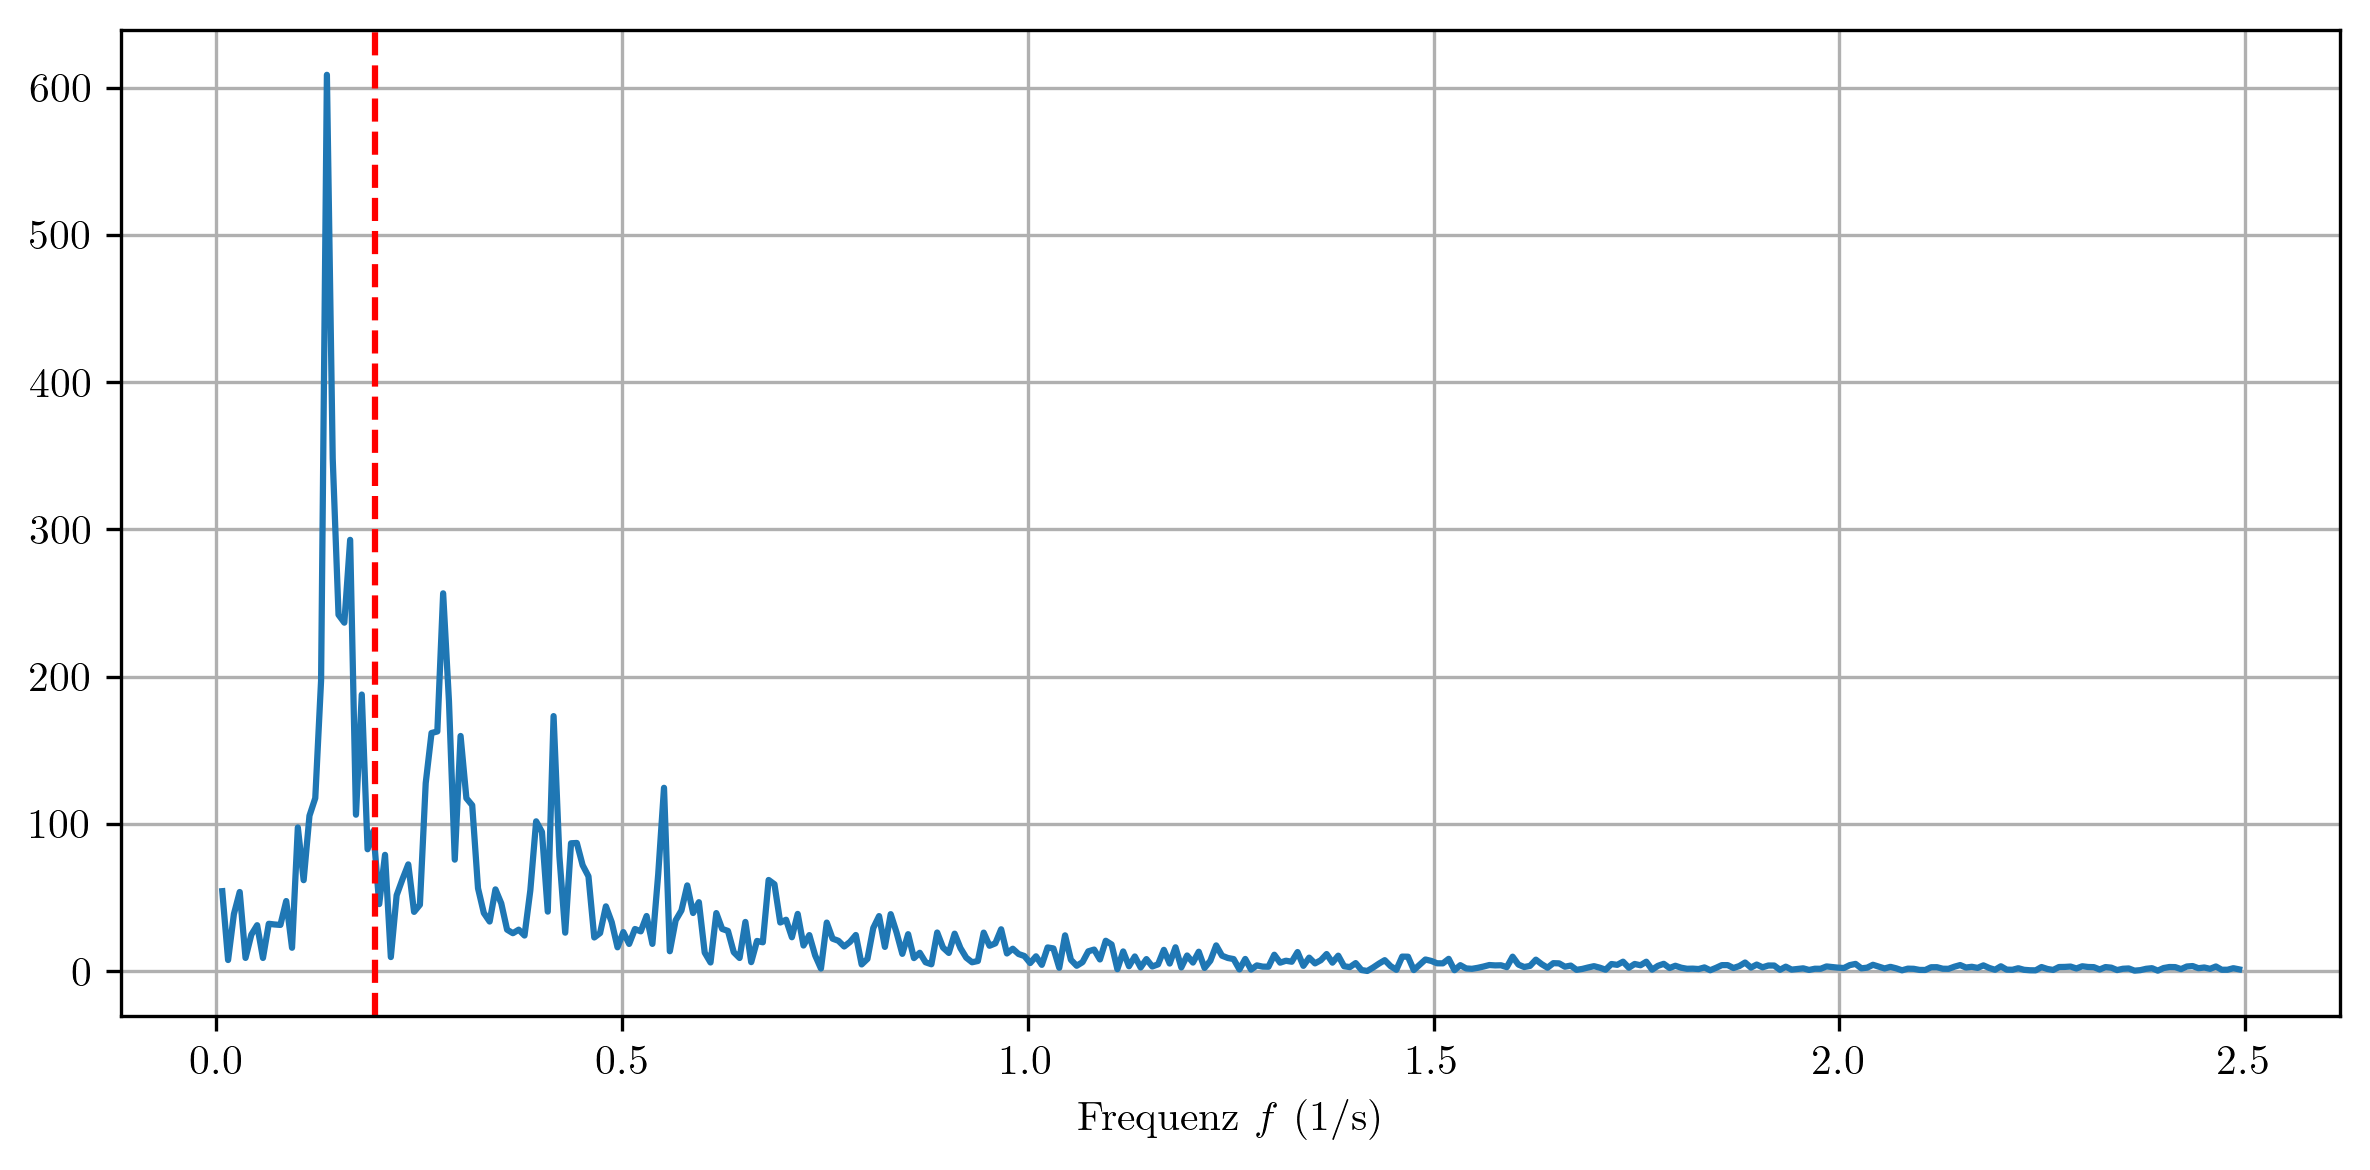
\includegraphics[width=\linewidth]{papers/reaktdiff/images/LotkaVolterra/fft_plot_latex.png}
    \caption{FFT der Animation eines Reaktionsdiffusionsmodell mit den Reaktionstermen \eqref{reaktdiff:equation:lvsys}. Die rote Linie zeigt die theortisch dominante Frequnez von \(f = \omega / 2 \Pi \approx 0.195\,\text{Hz}\). Die Abweichung kann durch generelle abweichungen in der Simulation erklärt werden}
    \label{reaktdiff:fig:lvfft}
\end{figure}





